\documentclass{scrartcl}
\usepackage[a4paper,left=1in,right=1in,top=1.2in,bottom=1in]{geometry}
\usepackage{siunitx}
\usepackage{graphicx}
\setkomafont{disposition}{\normalfont\bfseries}

%title
\title{Exercise 09:\\Information theory}
\subtitle{Theoretical Neuroscience I}
\author{Maria del Cerro \and Johannes G\"atjen \and Lorena Morton}

%use these for structure/overview
\newcommand\Question{%
  \textbf{Question:}%
}
\newcommand\Answer{%
  \textbf{Answer:}%
}

\begin{document}
\maketitle
\section{Assignment I: Count probability}

\begin{figure}[h]
\centering
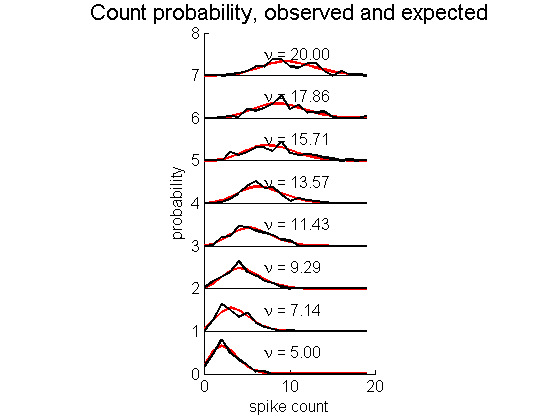
\includegraphics[trim = {1.3cm 0 1.5cm 0.1cm}, width=0.6\textwidth, clip]{../pics/as1}
\caption{The observed (black) and expected (red) count probability for the different conditions. The observed probabilities fit fairly well to the expected values. The differences can be attributed to the comparatively low number of samples used (100) and vanish with higher sample sizes.}
\label{as1}
\end{figure}

\section{Assignment III: identification performance}

We computed the reliability of correctly identifying the stimulus condition and compared the results to the theoretical value. Initial results are shown in Figure \ref{as3}. The theoretical and empirical results do not fit well together. In particular, the theoretical reliability peaks at $t=0.8\si{s}$, which does not make sense, because in theory, the longer you observe a Poisson process, the closer the measured spiking rate will be to the actual underlying value and you get a higher reliability. This is due to the fact, that when generating the \texttt{SpikeRaster} we set \texttt{Nspike=20}. This means, that even when there would have been more spikes before $t_0$, they are not generated and falsify the results. We repeated the calculations with \texttt{Nspike=200} to virtually guarantee, that spikes are never stopped generating prematurely. The results are shown in Figure \ref{as32}. As expected, the fraction correct now increases with time. The analytical solution is however higher than the empirical one, by what looks to be a constant factor. The reason for this is, that the empirical and the analytical solutions do not use consistent methods to calculate the fraction of correct identifications. A non-technical possible explanation could be, that for the theoretical calculation, all of the available information is concentrated into the single most likely result, whereas with the formula used for the empirical values the available information is distributed evenly among all candidates.

\begin{figure}
\centering
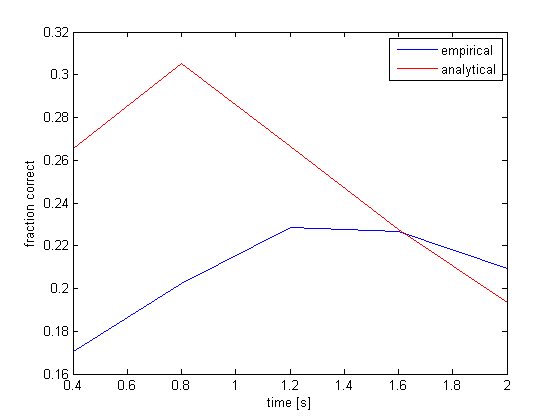
\includegraphics[trim = {0.6cm 0 1.2cm 0.7cm}, width=0.7\textwidth, clip]{../pics/as3}
\caption{The empirical (blue) and theoretical (red) fraction of correct identifications of the condition given a spike count, for \texttt{Nspike=20} and different values of $t_0$.}
\label{as3}
\end{figure}

\begin{figure}
\centering
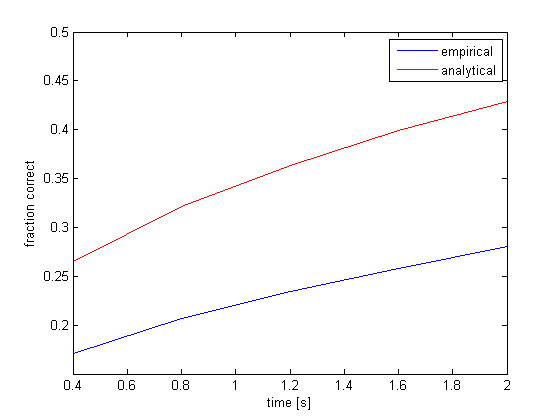
\includegraphics[trim = {0.6cm 0 1.2cm 0.7cm}, width=0.7\textwidth, clip]{../pics/as3_2}
\caption{The empirical (blue) and theoretical (red) fraction of correct identifications of the condition given a spike count, for \texttt{Nspike=200} and different values of $t_0$.}
\label{as3_2}
\end{figure}


%include picture
%\begin{figure}
%\centering
%\includegraphics[trim = {1.3cm 0 2cm 0.9cm}, width=\textwidth, clip]{../pics/picname}
%\caption{caption text}
%\label{label}
%\end{figure}
\end{document}